\documentclass[letterpaper,twocolumn,10pt]{article}

\usepackage{tikz}
\usepackage{amsmath}
\usepackage{graphicx}
\usepackage{float}
\usepackage{lipsum}
\usepackage{sidecap}
\usepackage{hyperref}
\usepackage{xcolor}

\usepackage{titling}

%\usepackage[left=0.5in,right=0.5in, bottom=0.5in]{geometry}
%\setlength{\droptitle}{-10em}
\usepackage[margin=0.5in]{geometry}



%-------------------------------------------------------------------------------
\begin{document}
% -------------------------------------------------------------------------------

\date{}

\title{Serial-Optimising Chessboard-Pattern Stenciling}

\author{
  {\rm Jan Fecht}\\
  University of Bristol}

\maketitle


% -------------------------------------------------------------------------------
\section*{Introduction}
% -------------------------------------------------------------------------------
The program to be optimized consists of a simple stencil applied on a chessboard-pattern image.
The user can specify the width ($nx$) and the height ($ny$) of the image and furthermore
the number of times that the stencil is applied ($niters$). All of these parameters are passed on the command line to the program, except for $niters$ which is passed as $niters/2$ instead.

For comparing and evaluating the effect of
a particular optimisation, the final version of the code was benchmarked
and compared to the final version without the optimization.

Most measured times were determined by taking the average of 100 runs
on the University's \textit{Blue Crystal 4} supercomputer (bc4). The times for
the original version were taken from the official repository instead
\footnote{ \url{https://github.com/UoB-HPC/intro-hpc-stencil/}} as running
it 100 times would have been infeasible.

The speedup of the final version can be seen in Table~\ref{tab:final}.  \\

\textbf{Disclaimer} The optimisations applied were neither introduced
in the order nor grouped together as they are described in this report. Rather, the 
whole optimisation process was iterative because new ideas and adaptions to new
circumstances were necessary. Therefore most comparisons were conducted by trying to remove
a whole set of small optimisations made that can be grouped together.

\begin{table}[ht]
	\caption{Final version compared to the original version ($niters=200$).}
	\begin{tabular}{c c c c}
		 image size & original & final & speedup \\
		 \hline
		1024 x 1024 & 5.908341s   & 0.01703819s & 346.77 \\
		4096 x 4096 & 130.196475s & 0.02655836s & 4902.28\\
		8000 x 8000 & 561.118133s & 0.04257847s & 13178.45\\
	\end{tabular}
	\label{tab:final}
\end{table}

% -------------------------------------------------------------------------------
\section*{Algorithm}
% -------------------------------------------------------------------------------
The chessboard pattern contains a high degree of symmetry and by applying the stencil code
to all points the original code performs plenty of redundant computations.
The number of floating point operations lies in $\Theta(nx * ny * niters)$
as the number of points to be stenciled is $nx * ny *niters$.
To reduce this number drastically, one can stencil only small parts of the image and apply
these precomputed parts to the whole image by copying and possibly mirroring and in the case
of the center inverting them. The specific parts that need to be precomputed can be seen
in Figure~\ref{fig:board} as the opaque fields. The center part in \textcolor{red}{red} cannot be applied to the whole image but only to the center in transparent red.
The reason for this lies in the way the borders are stenciled in the original version. It assumes that there is an invisible black border around the field. This lead to a slightly darker border which affect all pixels in a range of $niters$ around the border. This is marked as the \textcolor{green}{green}, \textcolor{blue}{blue} and \textcolor{yellow}{yellow} parts in Figure~\ref{fig:board}.

The \textcolor{blue}{blue} corners can only be reused for the \textcolor{yellow}{yellow} corners if they share the same colored (black or white) tile in the most outer part. This is only the case iff $nx + ny = 0 \text{ (mod } 128\text{)}$

If either $nx \neq 0 (mod 64)$ or $ny \neq 0 (mod 64)$, the right or lower border and all
corners
\begin{figure}[ht]
	\begin{center}
	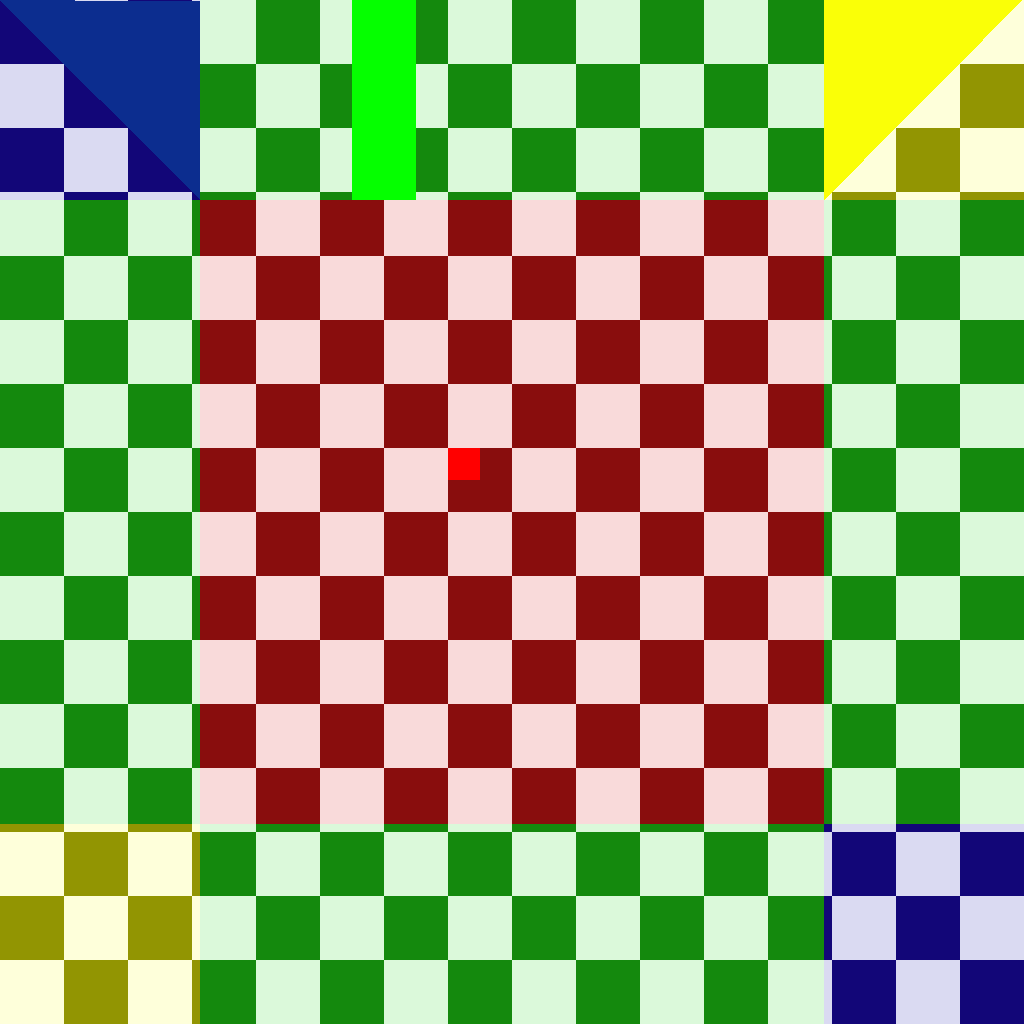
\includegraphics[width=150pt]{res/stencil_colored_with_prec}
	\caption{Colored 1024 x 1024 pattern assumming 100 iterations. Areas that need to be precomputed in opaque.}
	\end{center}
	\label{fig:board}
\end{figure}

\section*{Access Pattern}

\section*{Vectorisation}
- Alignment
- \_\_builtin\_assume\_aligned
- speedups
- replace memcpy with for loops

\section*{Other Improvements}
- compiler flags
- failed attempts

\section*{Further possible Improvements}

% -------------------------------------------------------------------------------
\section*{Conclusion}
% -------------------------------------------------------------------------------


\bibliographystyle{plain}
\bibliography{lit}

\end{document}
